% Transactions in big-data platforms
In recent years, transaction processing~\cite{Gray:1992:TPC:573304} technologies have paved their way into multi-petabyte big data 
platforms~\cite{Percolator2010,Spanner2012,Omid2017}. 
%In some cases, they are built into the storage system itself~\cite{Spanner2012} whereas in the others they are standalone services~\cite{Omid2017}. 
Modern industrial transaction processing systems~\cite{Percolator2010, Omid2017, tephra, cockroach} complement 
existing underlying NoSQL key-value storage with {\em atomicity}, {\em consistency}, {\em isolation\/} and {\em durability} (ACID) 
semantics that enable programmers to perform complex data manipulation without over-complicating their applications. 
Google's Percolator~\cite{Percolator2010} pioneered a transaction API atop the Bigtable storage. Apache 
Incubator projects Tephra~\cite{tephra} and Omid~\cite{Omid2017} followed suit with Apache HBase~\cite{hbase}. 

Adopting these technologies in new domains, in particular, real-time cloud analytics, raises three principal challenges: performance, functionality, and cloud-deployability, as we now explain.   

{\bf Performance.\ }
Similarly to many technologies, the adoption of transactions took a  ``functionality-first" trajectory. 
For example, the developers of Spanner~\cite{Spanner2012} wrote: 
%\begin{quote}
  ``We believe it
is better to have application programmers deal with performance problems due to overuse 
of transactions as bottlenecks arise, rather than always coding around the lack of transactions''. 
%\end{quote}
Yet the expectation for high performance is rapidly picking up. 
Whereas early transaction systems were  latency-insensitive~\cite{Percolator2010, Omid2017}, 
with the thrust into new interactive domains like social networks~\cite{chatter},  
messaging~\cite{Borthakur:2011} and algorithmic trading~\cite{opentsdb} latency becomes essential.  
SLAs for interactive user experience mandate that simple updates and point queries  complete within single-digit milliseconds. 
%Such applications motivate further speedup of transaction processing infrastructure. 

{\bf Functionality.\ }
Transaction support in huge-scale applications was initially motivated by specific use cases like content indexing for web search~\cite{Percolator2010, Omid2017} but  rapidly evolved into a wealth of OLTP and operational analytics 
applications (e.g.,~\cite{Borthakur:2011, F1-2013}). 
%Moreover, managing all data and insights in one place is becoming a prevalent requirement. 
A recent Forrester report~\cite{Forrester2017} coins the notion of {\em translytics}  as ``a unified and integrated data platform that supports multi-workloads such as transactional, operational and analytical simultaneously in real-time, ... and ensures full transactional integrity and data consistency''. Indeed, we see scalable data management platforms (e.g., Google Spanner~\cite{Spanner2012}, Apache Phoenix~\cite{phoenix}, and CockroachDB~\cite{cockroach}) shifting from NoSQL to full-fledged SQL interfaces in order to provide complex query semantics in conjunction with strong data guarantees. SQL support raises new requirements for transaction management, e.g., in the context of secondary index maintenance. 

{\bf Cloud-deployability.\ }
%Finally, 
Modern translytics platforms are built cloud-native. In particular, multi-tenancy becomes key 
for hosting data owned by multiple applications without breaching access rights. This requirement 
affects design choices made in the transaction processing system. 

% Drum roll 
{\bf Omid evolution.\ }
This paper describes recent functionality extensions and performance improvements 
we made in Omid~\cite{omid}, an open source transaction manager for HBase, to power 
Phoenix~\cite{phoenix},  a Hadoop SQL-compliant  data analytics platform designed 
for cloud deployment. In contrast to earlier SQL query engines for Hadoop (e.g., 
Hive~\cite{hive} and Impala~\cite{impala}), which focused on large-scale processing
of immutable data, Phoenix targets converged data ingestion and analytics~\cite{PhoenixUseCases},
which necessitates transaction semantics. Phoenix
applications are both latency- and throughput-sensitive. Phoenix uses HBase 
<<<<<<< HEAD
as key-value storage layer, and Omid as transaction processing layer\footnote{\small{Tephra 
is supported as alternative transaction manager, however its scalability and reliability are inferior to Omid.}}. 
=======
as its key-value storage layer, and \inred{is adopting Omid as} its transaction processing layer\footnote{
\small{Tephra is supported as alternative transaction manager, however its scalability 
and reliability are lower than Omid's.}}. 
>>>>>>> f944b4f0a698756f78eb687b182e8dd6212359d1

\remove{
Similarly to other modern transaction managers~\cite{Percolator2010,Spanner2012,tephra,cockroach}, it provides a (somewhat relaxed) 
variant of \emph{snapshot isolation (SI)}~\cite{DBLP:conf/sigmod/BerensonBGMOO95}, 
which scales better than traditional serializability implementations.}

This paper makes the following contributions: 
\begin{enumerate}
    \setlength{\itemsep}{1pt}
    \setlength{\parskip}{1pt}
    \setlength{\parsep}{1pt}  

\item {\em Protocol re-design for low-latency transactions}. 
The new protocol,  \sysll, dissipates a major architectural bottleneck. 
It reduces the latency of short transactions by 5x under light load, and 
by 10x-100x under heavy load compared to the legacy Omid. It also scales 
the overall system throughput to 550K transactions per second while remaining 
within real-time latency SLA's. In contrast to previously published protocols 
(e.g.,~\cite{Percolator2010}), our solution is amenable to multi-tenancy.

\item {\em Novel fast-path algorithm}. The  novel (experimental) \sys\ protocol  
maximizes the performance of  single-key transactions, which are prevalent 
in latency-sensitive applications. It defines a dedicated API for single-read, 
single-write and read-modify-write transactions.  Fast path transactions execute at the 
latency of native HBase operations regardless of system load.
%(thanks to HBase's near perfect horizontal scalability). 
<<<<<<< HEAD
They run twice as fast as \sysll\/ transactions, and complete within $2-4$ ms on mid-range hardware. 
This comes at the cost of a minor ($15-25\%$) negative impact on long (latency-insensitive) transactions.  
=======
They run twice as fast as \sysll\/ transactions, and complete within 2--4 ms on mid-range hardware. 
This comes at the cost of a minor (15--25$\%$) negative impact on long (latency-insensitive) transactions.  
>>>>>>> f944b4f0a698756f78eb687b182e8dd6212359d1

\item {\em SQL compliance\/}. We add support for creating 
secondary indices on-demand for accelerated analytics, without impeding concurrent database operations
or sacrificing consistency. 

\end{enumerate}

{\bf Roadmap.\ }
 Section~\ref{sec:api} defines  the service API and semantics. Section~\ref{sec:ll} describes \sysll, 
 our protocol redesign for improved performance with multi-tenancy support.  
Section~\ref{sec:alg} details our fast path algorithm, \sys.
We extensively evaluate the new algorithms in Section~\ref{sec:eval}.  
The functionality extensions are given in Section~\ref{sec:sql}.  
Section~\ref{sec:related} reviews related work, and  Section~\ref{sec:conclusions} concludes.


\remove{
\begin{figure}
  \centerline{
        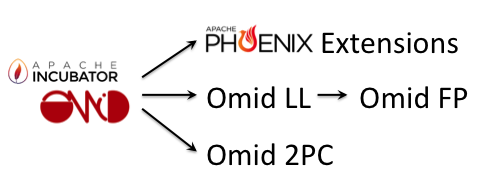
\includegraphics[width=0.75\columnwidth]{figs/OmidVersions}	
  }
\caption{
%Our extensions of Apache Incubator Omid. 
              We extend the  Apache Incubator version of Omid to support APIs  for SQL transactions in Phoenix. 
              In a complementary branch,
              we develop a low latency version \sysll, and extend it to support fast-path transactions in \sys.
              We also implement a variant based on two phase commit, \syspc, for comparison.}
\label{fig:evolution}
\end{figure}
}

\remove{
The performance  improvement  is achieved in two steps, as depicted in the middle row in  Figure~\ref{fig:evolution}.  
%by two design changes.
First, in Section~\ref{sec:ll}, we create a new low latency version of Omid, \sysll, which
dissipates Omid's principal bottleneck. It  
distributes persistent writes of transaction commit records, which is a centralized bottleneck in Omid. 
\sysll\ uses Omid's centralized transaction manager for timestamp allocation and conflict detection, 
but relieves it of performing I/O. 
%
For comparison, we implement a variant of Omid that uses Percolator's \emph{two-phase commit (2PC)} approach to 
conflict detection~\cite{Percolator2010}, which we call \syspc. 
\inred{
However, the Percolator approach  assumes that all transactions have permission 
to access all data tables, which is common in single-application settings, but is often not the case 
in multi-tenancy scenarios. \sysll\  instead, follows Omid's approach of storing conflict information in a common \emph{commit table}, which does  not  hold application data and is exclusively accessed by the transaction management layer.
}

Our second performance improvement is motivated by the observation that, in many production settings, single-key transactions are prevalent. \inred{For example, an in-house analysis of transactions processed by a major e-commerce company revealed that $70\%$ of transactions affected a single database key.} 
In Section~\ref{sec:alg} we introduce a novel \emph{fast path} algorithm for short single-key transactions, which 
executes short transactions without the begin/commit overhead,  almost as fast as native HBase operations. 
%This entails minor extensions to the underlying data store. 
We call the resulting system \sys. 
Note that the fast path is orthogonal to other protocol aspects, and can be supported in other 
transaction processing services. 
%, to enable local commits directly within the storage layer and verify the correctness of general 
%transactions in presence of such commits. 
\inred{We discussed the fact that it uses coprocessor and maybe say it is experimental, but neither seems essential to elaborate at the introduction level.}
}

\remove{
%We have implemented {\sys\/} %\footnote{\url{https://github.com/yonigottesman/incubator-omid/tree/localTransactions}} 
Our implementations are 
based on the open source Omid code\footnote{\url{https://omid.incubator.apache.org}}.
To support \syspc\ and \sys, we further extended  HBase  to enable locking and the fast path, resp. 
%\footnote{\url{https://github.com/yonigottesman/hbase_local_transactions/tree/0.98-add-rmw}}. 
Our code is publicly available on github\footnote{\small{Omitted for blind review.}}
and since \sysll\ does not require HBase extensions.
\inred{We hope to contribute it back to the Omid open-source project.}
%and we are currently productionalizing \sysll, (which does not require HBase extensions),  
%and contributing the changes back to the Omid open-source project.
 }
 
 \remove{
 \inred{ 
 During our integration of Omid in Apache Phoenix, we came across the need to extend Omid's API in order
 to support certain SQL features, such as index building and  snapshots (Ohad, what was the name for that?). 
Section TBD describes the functionality extensions added in order to integrate Omid in Apache Phoenix. These extensions are currently implemented in a separate branch that has been integrated in Phoenix. They are complementary to the performance improvements of \sysll\ and \sys, which we also plan to integrate into the Phoenix branch in the future.
}
 
 Section~\ref{sec:eval} presents our experiments on mid-range hardware, which show substantial performance improvements.
Under low load, \sysll\ transactions are 4x to 5x faster than Omid's, 
and \sys\ further reduces the latency of short transactions by another $55\%$ on average.
As system load increases, Omid's latency surges (at  $\sim\!\!\!150$K tps in our tests),  
whereas \sys's remains stable. \syspc\ performs similarly to \sysll, except on long transactions
where it is slower; e.g., on $10$-key transactions \syspc\ is $30\%$ slower than \sysll.
% until we generate a higher load ($\sim\!\!500$K tps)
%, and increases four-fold at 500K tps.  
Fast path transactions incur no scalability
bottlenecks, and execute at the low latency of native HBase operations regardless of system load
(thanks to HBase's near perfect horizontal scalability).
This comes at the cost of a minor (15-25\%) negative impact on longer transactions. 
%{\inred{The system scales beyond 1M transactions per second on medium-end hardware,
%which surpasses Omid at least 4x.}} 
Additionally, \sys\ has negligible impact on  transaction abort rates.

\remove{
% \Idit{The roadmap below is not essential; maybe replace with summary of contributions.}
%The remainder of this paper is organized as follows:
In Section~\ref{sec:api} we define the  API and semantics of a transaction processing service. 
Section~\ref{sec:ll} describes \sysll, and 
%Section~\ref{sec:ha} discusses its high availability mechanism. 
Section~\ref{sec:alg} presents \sys.  Our evaluation is reported in 
Section~\ref{sec:eval}.
%In Section~\ref{sec:context} we generalize the fast path algorithm, and explain how it could be implemented in other systems. 
}

We review related work in Section~\ref{sec:related} and conclude with Section~\ref{sec:conclusions}.
In summary, our contributions are as follows:
\begin{enumerate}
    \setlength{\itemsep}{1pt}
    \setlength{\parskip}{1pt}
    \setlength{\parsep}{1pt}  
\item We extend Omid with functionality that facilitates implementing a SQL API and integrate it in Apache Phoenix.
\item We implement \sysll, a low-latency distributed transaction engine \inred{amenable to multi-tenancy}. 
%we plan to contribute it  to the Apache Omid project.
%which improves latency by 5x and doubles throughput; 
%we are working to incorporate in  production;
%\item We explore the design space of transaction processing engines for NoSQL data stores, 
%highlighting the tradeoffs between various design choices.  
\item We design a novel fast path for short transactions and implement it in \sys.
\item We extensively evaluate the new algorithms.
\end{enumerate}
}